\documentclass[10pt]{beamer}

\usepackage[utf8]{inputenc}
\usepackage[T1]{fontenc}
\usepackage{amsmath,amssymb, mathrsfs,stmaryrd}
\usepackage{dsfont}\let\mathbb\mathds
\usepackage[english]{babel}
\usepackage[all]{xy}
\usepackage{tikz-cd}
\usetikzlibrary{calc}
\usepackage{pgfplots}  

\institute{IBM Research Zurich\\ Université de Rennes 1}
\title[On Oriented Supersingular Isogeny Diffie-Hellman]{On Oriented Supersingular Isogeny Diffie-Hellman (Col\`{o} and Kohel, 2019)}
\author{Pierrick Dartois \\ Under the supervision of Luca De Feo}
\titlegraphic{
\includegraphics[width=3.5cm]{logo_IBM.png}\hspace*{1.75cm}~%
   
\includegraphics[width=3.5cm]{logo_Rennes1.jpg}
}

\date{September 1 2021}

%\AtBeginSection[]
   %{
   %\begin{frame}
   %\tableofcontents[currentsection]
   %\end{frame}
%}

\AtBeginSection[]{
  \begin{frame}
  \vfill
  \centering
  \begin{beamercolorbox}[sep=8pt,center,shadow=true,rounded=true]{title}
    \usebeamerfont{title}\insertsectionhead\par%
  \end{beamercolorbox}
  \vfill
  \end{frame}
}

\addtobeamertemplate{navigation symbols}{}{%
    \usebeamerfont{footline}%
    \usebeamercolor[fg]{footline}%
    \hspace{1em}%
    \insertframenumber/\inserttotalframenumber
}

\usepackage{graphicx} 

\usetheme{Warsaw}

\usepackage{mathtools}

%\theoremstyle{definition}
%\newtheorem{definition}{Definition}

\theoremstyle{plain}
\newtheorem{proposition}{Proposition}
%\newtheorem{lemma}{Lemma}
%\newtheorem{corollary}{Corollary}
%\newtheorem{theorem}{Theorem}

\theoremstyle{definition}
\newtheorem{remark}{Remark}
%\newtheorem{example}{Example}

\usepackage{pgf,tikz}
\usetikzlibrary{arrows}

%To set line spacing
\usepackage{setspace}
% To cross text
\usepackage{ulem}

%macros
\newcommand{\ie}{\emph{i.e.}\ }
\newcommand{\eg}{\emph{e.g.}\ }
\newcommand{\N}{\mathbb{N}}
\newcommand{\Z}{\mathbb{Z}}
\newcommand{\Q}{\mathbb{Q}}
\newcommand{\R}{\mathbb{R}}
\newcommand{\C}{\mathbb{C}}
\newcommand{\K}{\mathbb{K}}
\newcommand{\F}{\mathbb{F}}
\newcommand{\Hc}{\mathbb{H}}
\newcommand{\Lc}{\mathbb{L}}
\newcommand{\M}{\mathbb{M}}
\newcommand{\Pc}{\mathbb{P}}
\newcommand{\A}{\mathbb{A}}
\newcommand{\B}{\mathbb{B}}
\newcommand{\E}{\mathbb{E}}
\newcommand{\V}{\mathbb{V}}
\newcommand{\m}[1]{\mathcal{#1}}
\newcommand{\mA}{\mathcal{A}}
\newcommand{\mB}{\mathcal{B}}
\newcommand{\mC}{\mathcal{C}}
\newcommand{\mP}{\mathcal{P}}
\newcommand{\mK}{\mathcal{K}}
\newcommand{\mL}{\mathcal{L}}
\newcommand{\mE}{\mathcal{E}}
\newcommand{\mD}{\mathcal{D}}
\newcommand{\mF}{\mathcal{F}}
\newcommand{\mO}{\mathcal{O}}
\DeclareMathOperator{\im}{im}
%\renewcommand{\ker}{\mbox{ker}}
%\renewcommand{\dim}{\mbox{dim}}
%\renewcommand{\deg}{\mbox{deg}}
\renewcommand{\i}[2]{\left\llbracket #1~;~#2\right\rrbracket}
\renewcommand{\(}{\left(}
\renewcommand{\)}{\right)}
\renewcommand{\P}{\mathbb{P}}
%commandes de Quentin
%\newcommand{\F}[1]{\mathbb{F}_{#1}}
\newcommand{\Fp}[1]{\mathbb{F}_{p^{#1}}}
\newcommand{\db}[1]{\mathbb{#1}}
\newcommand{\id}{\mbox{id}}
\newcommand{\mf}[1]{\mathfrak{#1}}
\newcommand{\mfm}{\mathfrak{m}}
\newcommand{\mfn}{\mathfrak{n}}
\newcommand{\mfp}{\mathfrak{p}}
\newcommand{\mfq}{\mathfrak{q}}
\DeclareMathOperator{\Spec}{Spec}
\DeclareMathOperator{\Proj}{Proj}
\DeclareMathOperator{\Hom}{Hom}
\DeclareMathOperator{\End}{End}
\DeclareMathOperator{\Aut}{Aut}
\DeclareMathOperator{\Tr}{Tr}
\DeclareMathOperator{\disc}{disc}
\DeclareMathOperator{\Cl}{Cl}
\let\SS\relax
\DeclareMathOperator{\SS}{SS}
\DeclareMathOperator{\Ell}{Ell}
%\DeclareMathOperator{\mod}{mod}
\DeclareMathOperator{\Gal}{Gal}
\DeclareMathOperator{\nrd}{nrd}
\DeclareMathOperator{\Vol}{Vol}
\DeclareMathOperator{\Covol}{Covol}
\DeclareMathOperator{\lcm}{lcm}
\DeclareMathOperator{\ProjEval}{ProjEval}
\DeclareMathOperator{\Char}{char}%\char already taken
\DeclareMathOperator{\DL}{DL}
\DeclareMathOperator{\argmax}{argmax}

\newcommand{\leftmapsto}{\leftarrow\!\shortmid}
\newcommand{\longleftmapsto}{\longleftarrow\!\shortmid}
\renewcommand{\vec}[1]{\mathbf{#1}}


\begin{document}

\begin{frame}
\titlepage
\end{frame}

\begin{frame}
\tableofcontents
\end{frame}

\section{Introduction}

\subsection{Presentation of IBM Research}

\begin{frame}
% 3000 poeple in 12 countries 
\textbf{Key research areas in IBM Research}

\begin{columns}[t]
\column{.5\textwidth}
\begin{figure}
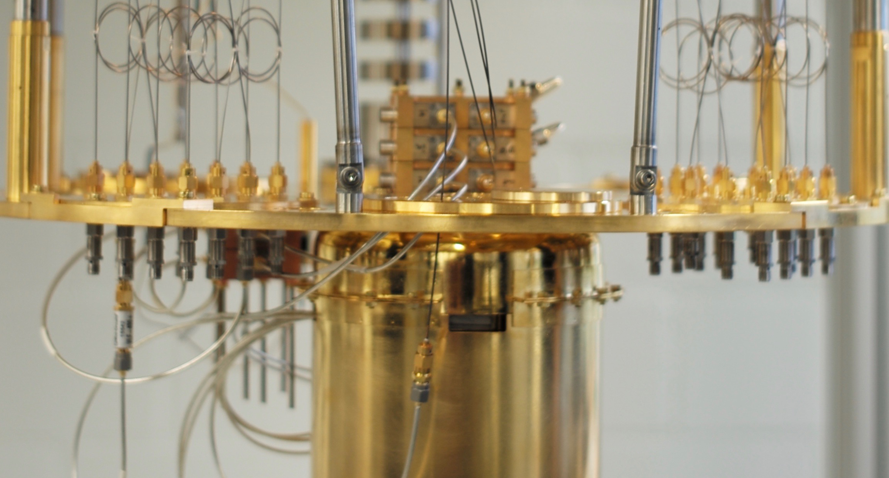
\includegraphics[width=3.5cm]
{science_and_technology.png} 

Science and Technology

\vspace{0.1cm}

{\setstretch{0.5} {\footnotesize Quantum computing, nanotechnologies, semi-conductors, electronics,  green technologies...}\\}
\vspace{0.3cm}


\includegraphics[width=3.5cm]
{security.jpg} 

Security

\vspace{0.1cm}

{\setstretch{0.5} {\footnotesize Post-quantum cryptography, blockchain, cybersecurity, identity and data governance...}\\}


\end{figure}


\column{.5\textwidth}

\begin{figure}

\includegraphics[width=3.5cm]
{cloud_and_AI.png} 

Cloud and AI

\vspace{0.1cm}

{\setstretch{0.5}{\footnotesize Machine learning, hardware technologies for storage, memory and processing in the cloud...}\\}

\vspace{0.3cm}


\includegraphics[width=3.5cm]
{cognitive_computing.jpg}

Cognitive computing

\vspace{0.1cm}

{\setstretch{0.5}{\footnotesize Computational biology and medicine, supercomputing, predictive maintenance...}\\}

\vspace{0.05 cm}

{\tiny Pictures by IBM}
\end{figure}
\end{columns}

\end{frame}

%\subsection{Contextualization of OSIDH}

\subsection{Post quantum and isogeny based cryptography}

\begin{frame}
\textbf{Quantum computers are a threat to current cryptography}

\begin{itemize}
\item Shor's algorithm (1995) can compute discrete logarithms and factor integers in polynomial time on a quantum computer.

\item All current public key cryptography based on these problems may become unsafe (\sout{RSA} and \sout{El Gamal}).
\end{itemize}

\begin{columns}[t]
\column{.3\textwidth}

\begin{figure}
\includegraphics[width=3cm]{quantum_computer.png} 
{\tiny Picture by IBM}
\end{figure}


\column{.7\textwidth}

\begin{figure}
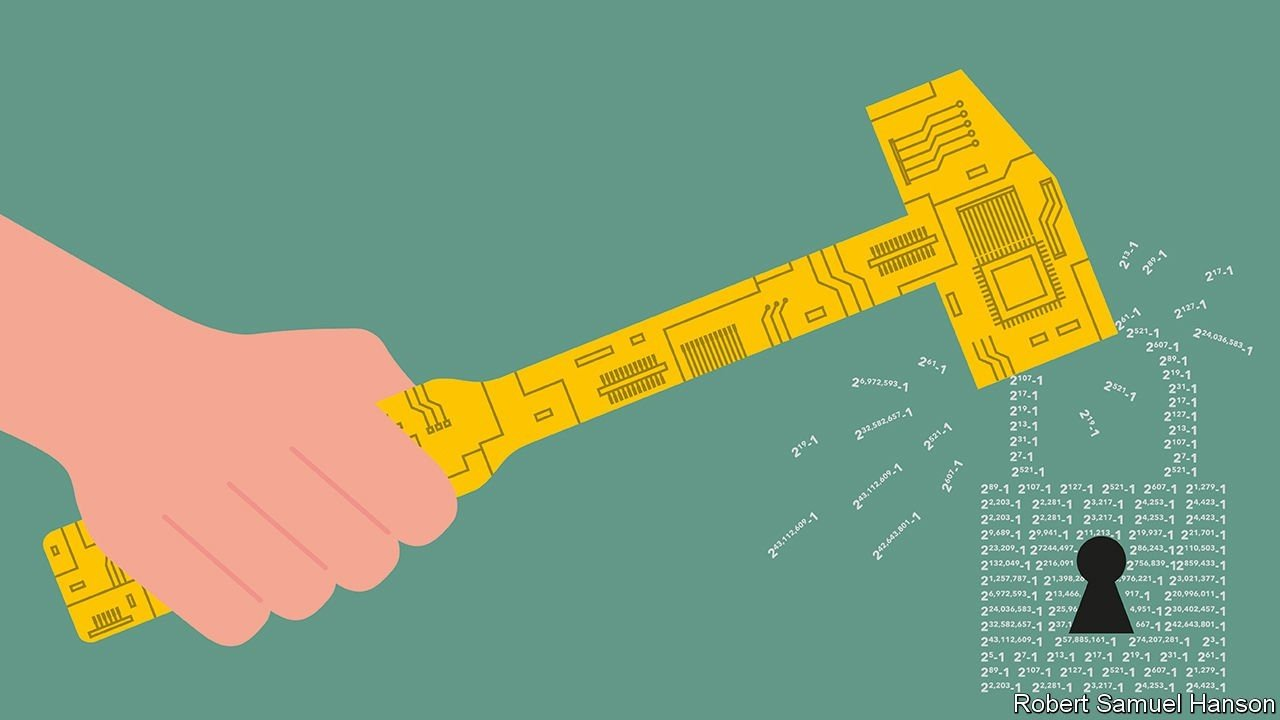
\includegraphics[width=6cm]{hammer.jpeg} 

{\tiny Picture by Robert Samuel Hanson}
\end{figure}


\end{columns}

\end{frame}



\begin{frame}
\textbf{Isogeny based cryptography in the NIST competition}


\begin{figure}
\begin{columns}[t]
\column{.5\textwidth}


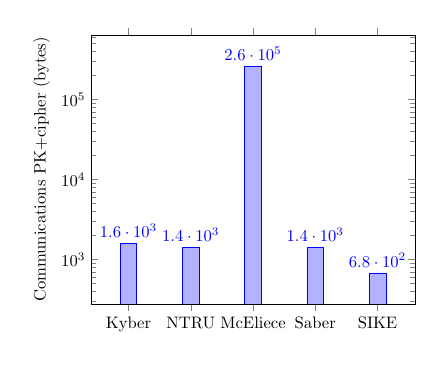
\begin{tikzpicture}[scale=0.6]
  
\begin{axis}  
[  
    ybar,  
    ymode=log,
    enlargelimits=0.15,  
    ylabel={Communications PK+cipher (bytes)}, % the ylabel must precede a # symbol.  
    %xlabel={},  
    symbolic x coords={Kyber, NTRU, McEliece, Saber, SIKE}, % these are the specification of coordinates on the x-axis.  
    xtick=data, 
    point meta=rawy,
     nodes near coords={\pgfmathprintnumber[sci,precision=1]{\pgfplotspointmeta}}, % this command is used to mention the y-axis points on the top of the particular bar.  
    nodes near coords align={vertical},  
    ]  
\addplot coordinates {(Kyber,1568) (NTRU,1398) (McEliece,261248) (Saber,1408) (SIKE,676) };  
  
\end{axis}  
\end{tikzpicture} 
\column{.5\textwidth}


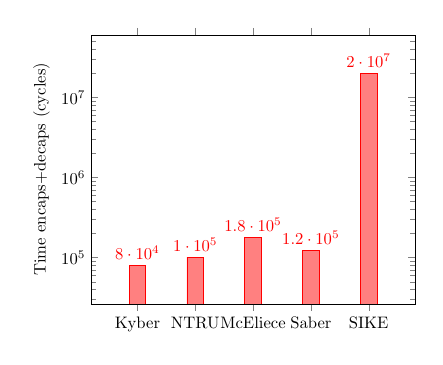
\begin{tikzpicture}[scale=0.6]
  
\begin{axis}  
[  
    ybar,  
    ymode=log,
    enlargelimits=0.2,  
    ylabel={Time encaps+decaps (cycles)}, % the ylabel must precede a # symbol.  
    %xlabel={},  
    symbolic x coords={Kyber, NTRU, McEliece, Saber, SIKE}, % these are the specification of coordinates on the x-axis.  
    xtick=data,  
    point meta=rawy,
     nodes near coords={\pgfmathprintnumber[sci,precision=1]{\pgfplotspointmeta}}, % this command is used to mention the y-axis points on the top of the particular bar.  
    nodes near coords align={vertical},  
    ]  
\addplot[color=red,fill=red!50] coordinates {(Kyber,79772) (NTRU,101357) (McEliece,179095) (Saber,124000) (SIKE,20024000) };  
  
\end{axis}  
\end{tikzpicture}


\end{columns}

\caption{Total communication size (public key and cipher) and time performance (encapsulation and decapsulation) of 5 NIST round 3 key encapsulation mechanisms.}
\end{figure}

\end{frame}

\subsection{Cryptographic group actions and Diffie-Hellman key exchange}


\begin{frame}
\textbf{Cryptographic group action}\footnote[frame]{Brassard and Yung (1991), Couveignes (2006).}

\vspace{0.5cm}

\begin{itemize}
\item $G$: an abelian group.
\item $X$: a set ($|X|=|G|$).
\pause 
\item $\cdot : G\times X\longrightarrow X$ a \emph{transitive} and \emph{faithful} group action:
\[\forall x,y\in X, \exists g\in G, \quad g\cdot x=y \quad (\mbox{transitivity})\]
\[\forall x\in X,  g\in G, \quad g\cdot x=x \Longrightarrow g=e \quad (\mbox{faithfulness})\]
\pause
\item Group action easy to compute.
\item \emph{One way} group action: hard to guess $g\in G$, with the knowledge of $x\in X$ and $g\cdot x$.
\end{itemize}

\end{frame}

\begin{frame}
\textbf{Diffie-Hellman key exchange}

\vspace{0.5cm}

\begin{itemize}
\item Public parameter: $x_0\in X$.
\item Alice's secret: $g\in G$.
\item Bob's secret: $h\in G$.
\end{itemize}

\pause

\begin{columns}[t]
\column{.4\textwidth}


\[\xymatrix{
x_0 \ar[d]^{h} \ar[r]^{g} & g\cdot x_0 \ar[d]^{h} \\
h\cdot x_0 \ar[r]^{g} & (gh)\cdot x_0
}\]


\column{.6\textwidth}

\begin{tikzpicture}[scale=1]

  \tikzstyle{every node}=[transform shape];

  % Alice
  \node (Alice) at (0,0) {
\includegraphics[height=2cm]{Alice.jpg}};
  \node (label) at (0,-1.5) {Alice};
  \node (label) at (0,-1.8) {{\tiny By Gallery Yopriceville}};
  
  % Bob
  \node (Bob) at (4,0) {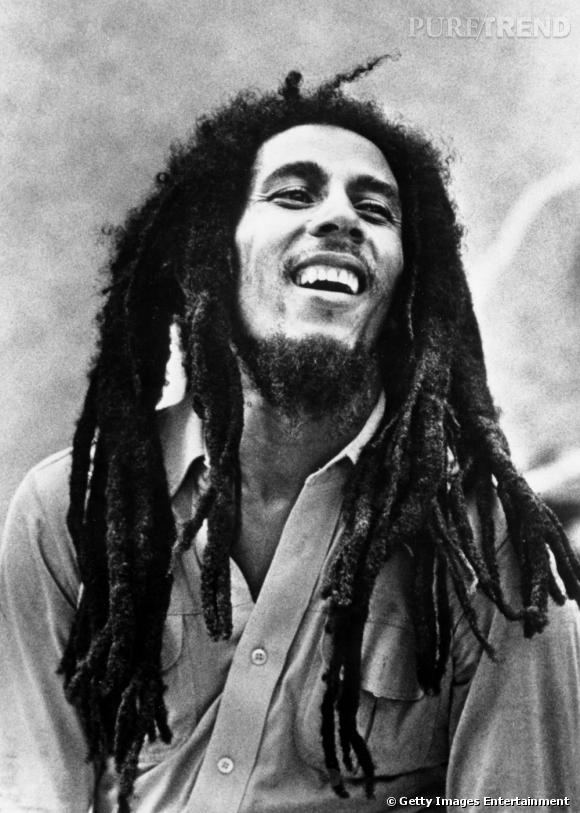
\includegraphics[height=2cm]{Bob.jpg}};
  \node (label) at (4,-1.5) {Bob};
  \node (label) at (4,-1.8) {{\tiny By Michael Ochs}};

% Messages
\draw[->,thick] ($(Alice)+(0.5,0.25)$) -- ($(Bob)+(-0.75,0.25)$) node [pos=0.5,above,font=\footnotesize] {$g\cdot x_0$};
\draw[->,thick] ($(Bob)+(-0.75,-0.25)$) -- ($(Alice)+(0.5,-0.25)$) node [pos=0.5,above,font=\footnotesize] {$h\cdot x_0$};

\end{tikzpicture}

\end{columns}

\end{frame}
%Show cryptographic group action, Couveignes cryptosystem, CSIDH, OSIDH.

\section{Mathematical framework of OSIDH}

\subsection{Orientations}

\begin{frame}
\textbf{Oriented elliptic curves}

\vspace{0.5cm}

\begin{itemize}
\item $K$: quadratic imaginary field.
\item $\mO$: order of $K$.
\item $E/\F_q$: elliptic curve.
\end{itemize}

\begin{definition}[Col\`{o} and Kohel]
A $K$-\emph{orientation} of $E$ is an embedding: 
\[\iota : K\hookrightarrow \End(E)\otimes_\Z\Q.\]

$(E, \iota)$ is an $\mO$-\emph{orientation} if $\iota(\mO)\subseteq \End(E)$.  

It is \emph{primitive} if $\iota(\mO)=\End(E)\cap\iota(K)$.
\end{definition}

\pause

\begin{itemize}
\item If $E$ is ordinary, then $\iota(K)=\End(E)\otimes_\Z\Q$. Not very interesting.

\pause
\item If $E$ is supersingular, $\End(E)$ is a maximal order in a quaternion algebra: infinitely many possible orientations.
\end{itemize}

\end{frame}

\begin{frame}
\textbf{$K$-oriented isogenies}

\vspace{0.5cm}

\begin{itemize}
\item $(E, \iota)$ is a $K$-oriented elliptic curve. 
\item $\varphi : E\longrightarrow F$ is an isogeny.
\item We define a $K$-orientation $\varphi_*(\iota)$ on $F$ by:
\[\forall \alpha\in K,  \quad \varphi_*(\iota)(\alpha)=\frac{1}{\deg(\varphi)}\varphi\circ \iota(\alpha)\circ \widehat{\varphi}.\]
\end{itemize}

\begin{definition}[Col\`{o} and Kohel]
Let $(E, \iota_E)$ and $(F,\iota_F)$ be two $K$-oriented elliptic curves.  

An isogeny $\varphi : E\longrightarrow F$ is $K$-\emph{oriented} if $\varphi_*(\iota_E)=\iota_F$.  

We denote this by $\varphi : (E, \iota_E)\longrightarrow(F,\iota_F)$.
\end{definition}

\end{frame}

\begin{frame}
\textbf{Ascending, horizontal, descending $K$-oriented isogenies}

\vspace{0.5cm}

\begin{columns}[t]
\column{.51\textwidth}

\begin{itemize}
\item $\varphi : (E, \iota_E)\longrightarrow(F,\iota_F)$, a $K$-oriented isogeny.
\item $\mO:=\iota_E^{-1}(\End(E))$.
\item $\mO':=\iota_F^{-1}(\End(F))$.

\pause
\item If $\mO\subseteq\mO'$, then $\varphi$ is \emph{ascending}.
\item If $\mO=\mO'$, then $\varphi$ is \emph{horizontal}.
\item If $\mO\supseteq\mO'$, then $\varphi$ is \emph{descending}.
\end{itemize}

\column{.49\textwidth}

\definecolor{ffqqqq}{rgb}{1,0,0}
\definecolor{qqqqff}{rgb}{0,0,1}
\begin{tikzpicture}[line cap=round,line join=round,>=triangle 45,x=1cm,y=1cm,scale=0.7]
\clip(-3.5,-2.5) rectangle (3.5,1);
\draw [->,line width=1pt] (-1,0) -- (1,0);
\draw [->,line width=1pt,color=qqqqff] (-2,-2) -- (-1,0);
\draw [->,line width=1pt,color=ffqqqq] (1,0) -- (2,-2);
\begin{scriptsize}
\draw [fill=black] (-1,0) circle (2.5pt);
\draw[color=black] (-1.2,0.2) node {$\mathcal{O}$};
\draw [fill=black] (1,0) circle (2.5pt);
\draw[color=black] (1.2,0.2) node {$\mathcal{O}$};
\draw [fill=black] (-2,-2) circle (2.5pt);
\draw[color=black] (-2,-2.3) node {$\mathcal{O}'\subseteq\mathcal{O}$};
\draw [fill=black] (2,-2) circle (2.5pt);
\draw[color=black] (2,-2.3) node {$\mathcal{O}'\subseteq\mathcal{O}$};
\draw[color=black] (0,0.3) node {horizontal};
\draw[color=qqqqff] (-2.5,-1) node {ascending};
\draw[color=ffqqqq] (2.5,-1) node {descending};
\end{scriptsize}
\end{tikzpicture}

\end{columns}

\pause

\begin{proposition}[Kohel]
If $\ell:=\deg(\varphi)$ is prime, then: 
\begin{description}
\item[(i)] $\varphi$ is always ascending, horizontal or descending.
\item[(ii)] If $\varphi$ is ascending, then $[\mO':\mO]=\ell$.
\item[(iii)] If $\varphi$ is descending, then $[\mO:\mO']=\ell$.
\end{description}

\end{proposition}

\end{frame}

\subsection{Oriented supersingular isogeny graphs}

%\begin{frame}
%\textbf{$K$-oriented supersingular $\ell$-isogeny graphs}
%\vspace{0.5cm}
%\begin{itemize}
%\item $\ell$ and $p$ distinct prime numbers.
%\item $p$ does not split in $K$.
%\item \textbf{Vertices:} $K$-oriented supersingular elliptic curves defined over $\F_{p^2}$ up to $K$-oriented isomorphism.
%\item \textbf{Edges:} $K$-oriented isogenies of degree $\ell$.
%\end{itemize}

%\end{frame}

%\begin{frame}

%\textbf{The volcano structure}

%\vspace{0.5cm}

%\begin{proposition}[Kohel]
%Let $(E,\iota)$ be a supersingular primitively $\mO$-oriented elliptic curve and $\Delta_K:=\disc(K)$. Then:

%\begin{description}
%\item[(i)] If $\ell\nmid [\mO_K:\mO]$, among the $\ell$-isogenies with origin $(E,\iota)$:
%\begin{itemize}
%\item $1+\(\frac{\Delta_K}{\ell}\)$ are horizontal;
%\item $1/[\mO^\times:(\Z+\ell\mO)^\times]\(\ell-\(\frac{\Delta_K}{\ell}\)\)$ are descending;
%\item none of them are ascending.
%\end{itemize}

%\item[(ii)] If $\ell|[\mO_K:\mO]$, among the $\ell$-isogenies with origin $(E,\iota)$:
%\begin{itemize}
%\item none are horizontal;
%\item $\ell$ are descending;
%\item one of them are ascending.
%\end{itemize}
%\end{description}
%\end{proposition}

%\textbf{N.B.} These isogenies are considered up to $K$-oriented isomorphism.

%\end{frame}

\begin{frame}

\textbf{$K$-oriented supersingular $\ell$-isogeny graphs}

\vspace{0.5cm}

\textbf{Example:} $K=\Q(i)$, $\ell=2$, $p=79$,  $\F_{79^2}=\F_{79}[a]$ with $a^2-a+3=0$.

\begin{figure}[h!]
\centering

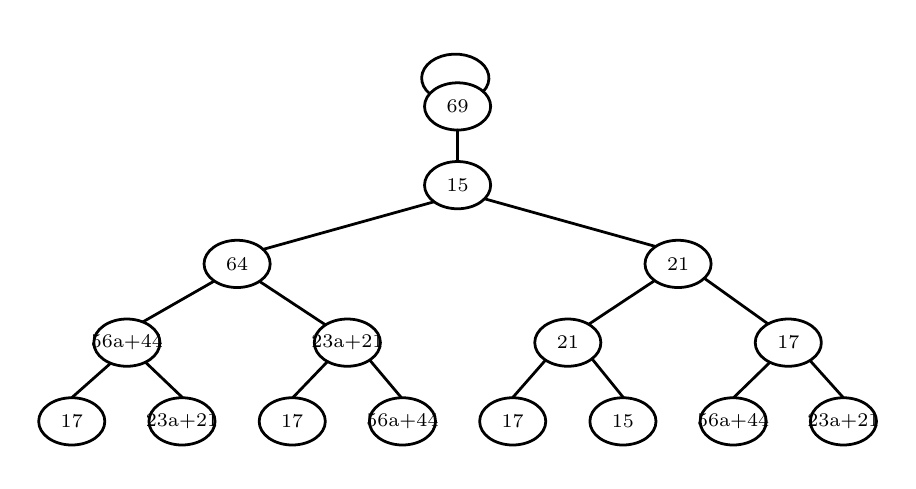
\begin{tikzpicture}[line cap=round,line join=round,>=triangle 45,x=1.4cm,y=1cm,scale=1]
\clip(-3.9,-4.5) rectangle (3.9,1);
\draw [line width=1pt] (3.5,-4) circle (0.3);
\draw [line width=1pt] (0,0) circle (0.3);
\draw [line width=1pt] (-1.5,-4) circle (0.3);
\draw [line width=1pt] (-3.5,-4) circle (0.3);
\draw [line width=1pt] (0.5,-4) circle (0.3);
\draw [line width=1pt] (2,-2) circle (0.3);
\draw [line width=1pt] (1.5,-4) circle (0.3);
\draw [line width=1pt] (-0.5,-4) circle (0.3);
\draw [line width=1pt] (-2.5,-4) circle (0.3);
\draw [line width=1pt] (-1,-3) circle (0.3);
\draw [line width=1pt] (-3,-3) circle (0.3);
\draw [line width=1pt] (0,-1) circle (0.3);
\draw [line width=1pt] (-2,-2) circle (0.3);
\draw [line width=1pt] (3,-3) circle (0.3);
\draw [line width=1pt] (1,-3) circle (0.3);
\draw [line width=1pt] (2.5,-4) circle (0.3);
\draw [line width=1pt] (0,-0.3)-- (0,-0.7);
\draw [line width=1pt] (-0.21322943610478404,-1.2110289259282618)-- (-1.763489092966821,-1.8154394656099442);
\draw [line width=1pt] (-1.7974860543853213,-2.2213325593571245)-- (-1.1980343823186057,-2.774650530465039);
\draw [line width=1pt] (-2.2067876385720067,-2.217345054081783)-- (-2.855544073501337,-2.7370694287470303);
\draw [line width=1pt] (-2.8316599983612933,-3.248317626938323)-- (-2.493627811564869,-3.700067682277239);
\draw [line width=1pt] (-3.1470895453233143,-3.261466375766714)-- (-3.5006593390669343,-3.70000072454755);
\draw [line width=1pt] (-1.18,-3.24)-- (-1.4957111195996629,-3.7000306590584437);
\draw [line width=1pt] (-0.797179438826777,-3.2210516228517196)-- (-0.5091578288571417,-3.70013980895987);
\draw [line width=1pt] (0.24489723766178567,-1.1732782242107382)-- (1.7970406198298907,-1.7790758274860692);
\draw [line width=1pt] (1.7876443158207822,-2.2119081484907466)-- (1.1890212652361931,-2.7670387128973815);
\draw [line width=1pt] (0.7978265785504022,-3.2216436501670267)-- (0.49846155869074266,-3.700003944695371);
\draw [line width=1pt] (1.2190320192368846,-3.2049999379244123)-- (1.5054935841881036,-3.700050303329428);
\draw [line width=1pt] (2.2379689093048514,-2.18267675879613)-- (2.8168942423162138,-2.7623610269693826);
\draw [line width=1pt] (3.1965297683390395,-3.2266628557055688)-- (3.5002064693248105,-3.700000071049312);
\draw [line width=1pt] (2.833538103582579,-3.249580522158913)-- (2.5028570132903156,-3.7000136045167067);
\draw [shift={(-0.020790003865610317,0.3591706988131075)},line width=1pt]  plot[domain=-0.5904004657771633:3.8476307905471328,variable=\t]({1*0.3052422908406379*cos(\t r)+0*0.3052422908406379*sin(\t r)},{0*0.3052422908406379*cos(\t r)+1*0.3052422908406379*sin(\t r)});
\begin{scriptsize}
\draw[color=black] (3.5,-4) node {23a+21};
\draw[color=black] (0,0) node {69};
\draw[color=black] (-1.5,-4) node {17};
\draw[color=black] (-3.5,-4) node {17};
\draw[color=black] (0.5,-4) node {17};
\draw[color=black] (2,-2) node {21};
\draw[color=black] (1.5,-4) node {15};
\draw[color=black] (-0.5,-4) node {56a+44};
\draw[color=black] (-2.5,-4) node {23a+21};
\draw[color=black] (-1,-3) node {23a+21};
\draw[color=black] (-3,-3) node {56a+44};
\draw[color=black] (0,-1) node {15};
\draw[color=black] (-2,-2) node {64};
\draw[color=black] (3,-3) node {17};
\draw[color=black] (1,-3) node {21};
\draw[color=black] (2.5,-4) node {56a+44};
\end{scriptsize}
\end{tikzpicture}
\end{figure}

\end{frame}

\begin{frame}

\textbf{Example:} $K=\Q(i)$, $\ell=2$, $p=79$,  $\F_{79^2}=\F_{79}[a]$ with $a^2-a+3=0$.

\vspace{0.3cm}

\textbf{The graph refolds!}

\begin{figure}[h!]
\centering

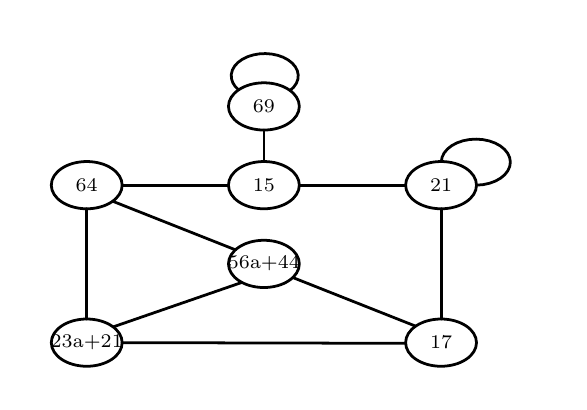
\begin{tikzpicture}[line cap=round,line join=round,>=triangle 45,x=1.5cm,y=1cm,scale=1]
\clip(-2,-3.5) rectangle (2.5,1);
\draw [line width=1pt] (0,0) circle (0.3);
\draw [line width=1pt] (0,-1) circle (0.3);
\draw [line width=1pt] (1.5,-1) circle (0.3);
\draw [line width=1pt] (-1.5,-1) circle (0.3);
\draw [line width=1pt] (1.5,-3) circle (0.3);
\draw [line width=1pt] (-1.5,-3) circle (0.3);
\draw [line width=1pt] (0,-2) circle (0.3);
\draw [line width=1pt] (0,-0.3)-- (0,-0.7);
\draw [line width=1pt] (0.3,-1)-- (1.2,-1);
\draw [line width=1pt] (1.5022058227240238,-1.2999918904672427)-- (1.5022058227240238,-2.7000081095327575);
\draw [line width=1pt] (1.2001241400766958,-3.0086295211488694)-- (-1.2,-3);
\draw [line width=1pt] (-1.5021428024802257,-1.2999923472316097)-- (-1.5021428024802257,-2.7000076527683903);
\draw [line width=1pt] (-1.2,-1)-- (-0.3,-1);
\draw [line width=1pt] (-1.2802410299272011,-1.2042204570373467)-- (-0.24099353148483596,-1.8213323818302058);
\draw [line width=1pt] (-0.18632449139731455,-2.235123762953752)-- (-1.2762572482543024,-2.80015210523685);
\draw [line width=1pt] (0.2449732494851846,-2.173170745325732)-- (1.2848736133624907,-2.79090519429625);
\draw [shift={(0.007090427603428667,0.3874717685141776)},line width=1pt]  plot[domain=-0.7124630393351774:3.8174613554669614,variable=\t]({1*0.2837279521520933*cos(\t r)+0*0.2837279521520933*sin(\t r)},{0*0.2837279521520933*cos(\t r)+1*0.2837279521520933*sin(\t r)});
\draw [shift={(1.7943119546152102,-0.7077247818460842)},line width=1pt]  plot[domain=-1.551337518465128:3.115189512445009,variable=\t]({1*0.2923305611926651*cos(\t r)+0*0.2923305611926651*sin(\t r)},{0*0.2923305611926651*cos(\t r)+1*0.2923305611926651*sin(\t r)});
\begin{scriptsize}
\draw[color=black] (0,0) node {69};
\draw[color=black] (0,-1) node {15};
\draw[color=black] (1.5,-1) node {21};
\draw[color=black] (-1.5,-1) node {64};
\draw[color=black] (1.5,-3) node {17};
\draw[color=black] (-1.5,-3) node {23a+21};
\draw[color=black] (0,-2) node {56a+44};
\end{scriptsize}
\end{tikzpicture}

\caption{Supersingular $2$-isogeny graph over $\F_{79^2}$.}
\end{figure}

\end{frame}

\begin{frame}
\textbf{Representing $K$-oriented elliptic curves by $j$-invariants}

\vspace{0.5cm}

\begin{itemize}
\item $\SS_K(p)$: set of $K$-oriented supersingular elliptic curves over $\F_{p^2}$ up to $K$-oriented isomomorphism.
\item $\SS(p)$: set of supersingular elliptic curves over $\F_{p^2}$ up to isomomorphism (supersingular $j$-invariants).
\item Unfortunately, the \emph{forgetful map}:
\[(E,\iota)\in\SS_K(p)\longmapsto E\in\SS(p)\]
is not injective.
\end{itemize}

\end{frame}

\begin{frame}
\textbf{Representing $K$-oriented elliptic curves by $j$-invariants}

\vspace{0.5cm}

\begin{itemize}
\item But we can restrict to $\mO$-orientations with $\disc(\mO)$ bounded.
\item $\SS_{\mO}(p)$: set of $\mO$-oriented supersingular elliptic curves over $\F_{p^2}$ up to $K$-oriented isomomorphism.
\end{itemize}

\begin{theorem}[Col\`{o} and Kohel]
If $p>|\disc(\mO)|$, then the forgetful map:
\[(E,\iota)\in\SS_{\mO}(p)\longmapsto E\in\SS(p)\]
is injective.
\end{theorem}

\end{frame}

\subsection{The ideal class group action}

\begin{frame}
\textbf{The ideal class group action}

\vspace{0.5cm}

\begin{itemize}
\item $\SS_{\mO}^{pr}(p)$: set of \textbf{primitively} $\mO$-oriented supersingular elliptic curves over $\F_{p^2}$ up to $K$-oriented isomorphism.
\item We define a group action:
\[\Cl(\mO)\times\SS_{\mO}^{pr}(p)\longrightarrow \SS_{\mO}^{pr}(p)\]
\item If $(E,\iota)\in \SS_{\mO}^{pr}(p)$ and $\mf{a}\subseteq\mO$ has norm prime to $p$, we consider:
\[\varphi_{\mf{a}}:E\longrightarrow E/E[\mf{a}]\]
with:
\[\ker(\varphi_{\mf{a}})=E[\mf{a}]:=\bigcap_{\alpha\in\mf{a}}\ker(\iota(\alpha))\]
\item We set:
\[[\mf{a}]\cdot (E,\iota):=(E/E[\mf{a}],(\varphi_{\mf{a}})_*(\iota))\]
\end{itemize}
\end{frame}

\begin{frame}
\textbf{The ideal class group action}

\vspace{0.5cm}

\begin{theorem}[Onuki]
The ideal class group action $\Cl(\mO)\times\SS_{\mO}^{pr}(p)\longrightarrow \SS_{\mO}^{pr}(p)$ is well-defined, \textbf{faithful} but \textbf{not transitive}. Actually, there are two orbits.
\end{theorem}

\vspace{0.5cm}

\pause

\textbf{To make it transitive:} restrict to the orbit of elliptic curves obtained by reduction mod $p$ of elliptic curves defined over a number field with complex multiplication by $\mO$. 

\end{frame}

\subsection{Chains and ladders}

\begin{frame}

\textbf{$\ell$-isogeny chains and ladders}

\begin{definition}
A $K$-oriented \emph{$\ell$-isogeny chain} of length $n$ is a sequence of $K$-oriented $\ell$-isogenies:
\[\xymatrix{
E_0 \ar[r]^{\varphi_0} & E_1 \ar[r]^{\varphi_{1}}& \cdots \ar[r]^{\varphi_{n-2}} & E_{n-1} \ar[r]^{\varphi_{n-1}} & E_n
}.\]

It is \emph{descending}, \emph{horizontal} or \emph{ascending} if all the $\varphi_i$ are.

\pause

A $K$-oriented \emph{$\ell$-ladder} of length $n$ and degree $q$ is a commutative diagram of $K$-oriented $\ell$-isogeny chains:
\[\xymatrix{
E_0 \ar[d]^{\psi_0} \ar[r]^{\varphi_0} & E_1\ar[d]^{\psi_1} \ar[r]^{\varphi_{1}}& \cdots \ar[r]^{\varphi_{n-2}} & E_{n-1} \ar[d]^{\psi_{n-1}} \ar[r]^{\varphi_{n-1}} & E_n \ar[d]^{\psi_n}\\
F_0 \ar[r]^{\varphi'_0} & F_1 \ar[r]^{\varphi'_{1}}& \cdots \ar[r]^{\varphi'_{n-2}} & F_{n-1} \ar[r]^{\varphi'_{n-1}} & F_n
}\]
such that $\psi_i : E_i\longrightarrow F_i$ is a $K$-oriented $q$-isogeny for all $i\in\i{0}{n}$.
\end{definition}

\end{frame}

%\begin{frame}
%\textbf{A useful $\ell$-ladder}

%\vspace{0.5cm}

%\begin{itemize}
%\item We set $\mO_i:=\Z+\ell^i\mO_K$ for all $i\in\i{0}{n}$.
%\item $q$: a splitting prime in $K$.
%\item $\mf{q}\subseteq \mO_K$: a prime ideal lying above $q$. 
%\item A descending $\ell$-isogeny chain:
%\[\xymatrix{
%E_0 \ar[r]^{\varphi_0} & E_1 \ar[r]^{\varphi_{1}}& \cdots \ar[r]^{\varphi_{n-2}} & E_{n-1} \ar[r]^{\varphi_{n-1}} & E_n
%}.\]
%with $E_0$, primitively $\mO_K$-oriented.
%\item There exists an $\ell$-ladder of degree $q$:
%\[\xymatrix{
%E_0 \ar[d]^{\psi_0} \ar[r]^{\varphi_0} & E_1\ar[d]^{\psi_1} \ar[r]^{\varphi_{1}}& \cdots \ar[r]^{\varphi_{n-2}} & E_{n-1} \ar[d]^{\psi_{n-1}} \ar[r]^{\varphi_{n-1}} & E_n \ar[d]^{\psi_n}\\
%F_0 \ar[r]^{\varphi'_0} & F_1 \ar[r]^{\varphi'_{1}}& \cdots \ar[r]^{\varphi'_{n-2}} & F_{n-1} \ar[r]^{\varphi'_{n-1}} & F_n
%}\]
%such that $F_i=[\mf{q}\cap\mO_i]\cdot E_i$ for all $i\in\i{0}{n}$.
%\end{itemize}

%\end{frame}

%\begin{frame}
%\textbf{How to compute the $\ell$-ladder:}
%\[\xymatrix{
%E_0 \ar[d]^{\psi_0} \ar[r]^{\varphi_0} & E_1\ar[d]^{\psi_1} \ar[r]^{\varphi_{1}}& \cdots \ar[r]^{\varphi_{n-2}} & E_{n-1} \ar[d]^{\psi_{n-1}} \ar[r]^{\varphi_{n-1}} & E_n \ar[d]^{\psi_n}\\
%F_0 \ar[r]^{\varphi'_0} & F_1 \ar[r]^{\varphi'_{1}}& \cdots \ar[r]^{\varphi'_{n-2}} & F_{n-1} \ar[r]^{\varphi'_{n-1}} & F_n
%}\]
%such that $F_i=[\mf{q}\cap\mO_i]\cdot E_i$ for all $i\in\i{0}{n}$, when the chain above is known?

%\vspace{0.5cm}

%\pause

%\begin{itemize}
%\item Compute the first $F_i$ with V\'{e}lu's formulas.
%\item Assuming $\Cl(\mO_K)=\{1\}$, trivial for $i=0$: $F_0=E_0$.
%\item For $i\geq i_0$ (such that $[\mfq\cap\mO_i]^2\neq [1]$), $j(F_{i})$ is the unique solution of:
%\[\left\{\begin{array}{c}
%\Phi_\ell(j(F_{i-1}),x)=0\\
%\Phi_q(j(E_{i}),x)=0.
%\end{array}\right. \]
%\end{itemize}

%\end{frame}

\begin{frame}
\textbf{Computing the ideal class group action in OSIDH}

\begin{columns}[t]
\column{.5\textwidth}

\begin{itemize}
\item $\mO_i:=\Z+\ell^i\mO_K$ for all $i\in\N$.
\item Represent an $\mO_n$-oriented elliptic curve $(E_n,\iota_n)$ by a descending $\ell$-isogeny chain $(E_i,\iota_i)_{0\leq i\leq n}$.
\item Let $\mfq\subseteq \mO_K$ be a prime ideal.
\item We compute the chain $(F_i,\iota'_i)_i:=[\mf{q}]\cdot (E_i,\iota_i)_i$:
\[\forall 0\leq i\leq n, \ F_i:=[\mf{q}\cap\mO_i]\cdot E_i\]
to get $F_n:=[\mf{q}\cap\mO_n]\cdot E_n$.
% descending the ladder.
\item Assumption: $\Cl(\mO_K)=\{1\}$, so that $E_0=F_0$.

\end{itemize}

\column{.5\textwidth}

\definecolor{qqwuqq}{rgb}{0,0.39215686274509803,0}
\definecolor{uuuuuu}{rgb}{0.26666666666666666,0.26666666666666666,0.26666666666666666}
\definecolor{xdxdff}{rgb}{0.49019607843137253,0.49019607843137253,1}
\definecolor{ududff}{rgb}{0.30196078431372547,0.30196078431372547,1}
\definecolor{violet}{rgb}{0.29411765,0,0.50980392}

%\begin{figure}[!h]
%\centering

\begin{tikzpicture}[line cap=round,line join=round,>=triangle 45,x=1cm,y=1cm,scale=0.5]
\clip(-3,-10.223333333333263) rectangle (7.5,3);
\draw [shift={(0,0)},line width=1pt,color=qqwuqq,fill=qqwuqq,fill opacity=0.10000000149011612] (0,0) -- (-89.9728461641534:5) arc (-89.9728461641534:-67.61733060429108:5) -- cycle;
\draw [line width=1pt,dash pattern=on 2pt off 5pt,color=violet] (0,0) circle (1cm);
\draw [line width=1pt,dash pattern=on 2pt off 5pt,color=violet] (0,0) circle (2cm);
\draw [line width=1pt,dash pattern=on 2pt off 5pt,color=violet] (0,0) circle (9cm);
\draw [line width=1pt,dash pattern=on 2pt off 5pt,color=violet] (0,0) circle (10cm);
\draw [line width=1pt] (0,0)-- (0.004739238223284909,-9.99999887698099);
\draw [line width=1pt] (0,0)-- (3.8079070583784587,-9.246612560000095);
\draw [shift={(0,0)},->,line width=1pt,color=qqwuqq] (-89.9728461641534:5) arc (-89.9728461641534:-67.61733060429108:5);
\begin{scriptsize}
\draw [fill=ududff] (0,0) circle (2.5pt);
\draw[color=ududff] (0.13,0.3666666666666649) node {$E_0$};
%\draw[color=black] (0,1.226666666666659) node {$\rho(\mbox{Ell}(\mathcal{O}_1))$};
%\draw[color=black] (0,2.286666666666652) node {$\rho(\mbox{Ell}(\mathcal{O}_2))$};
%\draw[color=black] (-2.4,-8.1) node {$\rho(\mbox{Ell}(\mathcal{O}_{n-1}))$};
%\draw[color=black] (-2.6,-9.2) node {$\rho(\mbox{Ell}(\mathcal{O}_n))$};
\draw [fill=xdxdff] (0.004739238223284909,-9.99999887698099) circle (2.5pt);
\draw[color=xdxdff] (-0.59,-9.673333333333268) node {$E_n$};
\draw [fill=uuuuuu] (0.0004739238223284909,-0.9999998876980991) circle (2pt);
\draw[color=uuuuuu] (-0.37,-0.6133333333333284) node {$E_1$};
\draw [fill=uuuuuu] (0.0009478476446569818,-1.9999997753961982) circle (2pt);
\draw[color=uuuuuu] (-0.33,-1.6333333333333215) node {$E_2$};
\draw [fill=uuuuuu] (0.0042653144009564175,-8.999998989282892) circle (2pt);
\draw[color=uuuuuu] (-0.64,-8.633333333333274) node {$E_{n-1}$};
\draw [fill=xdxdff] (3.8079070583784587,-9.246612560000095) circle (2.5pt);
\draw[color=xdxdff] (5.5,-9.5) node {$[\mathfrak{q}\cap\mO_n]\cdot E_n$};
\draw [fill=uuuuuu] (0.3807907058378459,-0.9246612560000096) circle (2pt);
\draw[color=uuuuuu] (1.7,-0.3333333333333304) node {$[\mathfrak{q}\cap\mO_1]\cdot E_1$};
\draw [fill=uuuuuu] (0.7615814116756918,-1.8493225120000192) circle (2pt);
\draw[color=uuuuuu] (2.2,-1.5) node {$[\mathfrak{q}\cap\mO_2]\cdot E_2$};
\draw [fill=uuuuuu] (3.427116352540613,-8.321951304000086) circle (2pt);
\draw[color=uuuuuu] (5.5,-7.8) node {$[\mathfrak{q}\cap\mO_{n-1}]\cdot E_{n-1}$};
\draw[color=qqwuqq] (1,-5.4) node {$\mathfrak{q}$};
\draw[color=violet] (1,1) node {$\mO_1$};
\draw[color=violet] (2.2,1.2) node {$\mO_2$};
\draw[color=violet] (2,-8.4) node {$\mO_{n-1}$};
\draw[color=violet] (2,-9.5) node {$\mO_n$};
\end{scriptsize}
\end{tikzpicture}

%\caption{Action of the prime ideal $\mfq$ on the descending $\ell$-isogeny chain.}
%\end{figure}
\end{columns}

\end{frame}

\section{The OSIDH protocol}

\subsection{A broken naive Diffie-Hellman protocol}

%\begin{frame}
%\textbf{General parameters:}
%\vspace{0.5cm}

%\begin{itemize}
%\item $K$: quadratic imaginary field such that $\Cl(\mO_K)=\{1\}$.
%\item $\ell$: prime number.
%\item $\mO_i:=\Z+\ell^i\mO_K$ for all $i\in\N$.
%\item $p$ does not split in $K$.
%\item $q_1, \cdots, q_t\neq \ell$ splitting primes in $K$.
%\item $\mfq_1, \cdots, \mfq_t$ primes of $\mO_K$ lying above $q_1, \cdots, q_t$.
%\item The $[\mfq_j\cap\mO_n]$ generate $\Cl(\mO_n)$.
%\end{itemize}

%\end{frame}

\begin{frame}
\textbf{Naive Diffie-Hellman key exchange:}
\vspace{0.5cm}

\textbf{Public parameters:}
\begin{itemize}
\item $q_1, \cdots, q_t\neq \ell$ splitting primes in $K$.
\item $\mfq_1, \cdots, \mfq_t$ primes of $\mO_K$ lying above $q_1, \cdots, q_t$.
\item The $[\mfq_j\cap\mO_n]$ generate $\Cl(\mO_n)$.
\item $(E_i)_{0\leq i\leq n}$ a public descending $\ell$-isogeny chain.
\end{itemize}

\vspace{0.5cm}

\begin{figure}[!h]
\centering

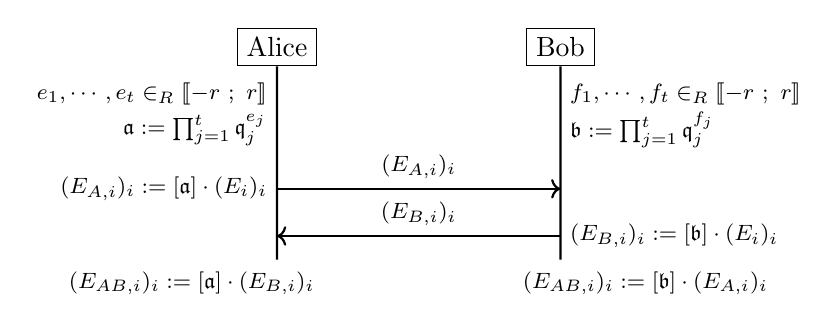
\begin{tikzpicture}[scale=0.6]
  % Public parameter:
  %\node[draw=none,fill=none,align=center] (public) at (0,1) {\footnotesize Public parameters:\\\footnotesize $(E_i)_i, \ \mf{q}_1, \cdots, \mf{q}_t$};
  
  % Alice
  \node[draw] (Alice) at (-3,0) {Alice}; 
  \draw[thick] (Alice) -- ++(0, -4.5);
    
  % Calculations of Alice
  \node[draw=none,fill=none,anchor=east] (asecret) at ($(Alice) + (0,-1)$) {\footnotesize $e_1,\cdots, e_t\in_R\i{-r}{r}$};
  \node[draw=none,fill=none,anchor=east] (asecretideal) at ($(Alice) + (0,-1.75)$) {\footnotesize $\mf{a}:=\prod_{j=1}^t\mf{q}_j^{e_j}$};
  \node[draw=none,fill=none,anchor=east] (Apublic) at ($(Alice) + (0,-3)$) {\footnotesize $(E_{A,i})_i:=[\mf{a}]\cdot (E_i)_i$};
  \node[draw=none,fill=none,anchor=east] (akey) at ($(Alice) + (1,-5)$) {\footnotesize $(E_{AB,i})_i:= [\mf{a}]\cdot (E_{B,i})_i$};
    
  % Bob
  \node[draw] (Bob) at (3,0) {Bob}; 
  \draw[thick] (Bob) -- ++(0, -4.5);
   
  % Calculations of Bob
  \node[draw=none,fill=none,anchor=west] (bsecret) at ($(Bob) + (0,-1)$) {\footnotesize $f_1,\cdots, f_t\in_R\i{-r}{r}$};
   \node[draw=none,fill=none,anchor=west] (bsecretideal) at ($(Bob) + (0,-1.75)$) {\footnotesize $\mf{b}:=\prod_{j=1}^t\mf{q}_j^{f_j}$};
  \node[draw=none,fill=none,anchor=west] (Bpublic) at ($(Bob) + (0,-4)$) {\footnotesize $(E_{B,i})_i:=[\mf{b}]\cdot (E_i)_i$};
  \node[draw=none,fill=none,anchor=west] (bkey) at ($(Bob) + (-1,-5)$) {\footnotesize $(E_{AB,i})_i:= [\mf{b}]\cdot (E_{A,i})_i$};
   
  % Messages
  \draw[->,thick] ($(Alice)+(0,-3)$) -- ($(Bob)+(0,-3)$) node [pos=0.5,above,font=\footnotesize] {\footnotesize $(E_{A,i})_i$};
  \draw[->,thick] ($(Bob)+(0,-4)$) -- ($(Alice)+(0,-4)$) node [pos=0.5,above,font=\footnotesize] {\footnotesize $(E_{B,i})_i$};
    
\end{tikzpicture}

\caption{Naive protocol.}
\end{figure}

\end{frame}

\subsection{Why is it broken?}

\begin{frame}
\textbf{Attack on the $\ell$-ladder}\footnote[frame]{Cl\`{o} and Kohel.}

\begin{columns}[t]
\column{.7\textwidth}

\begin{itemize}
\item Given $(E_i)_{i}$ and $(F_i)_i:=[\mf{a}]\cdot (E_i)_i$, we recover $[\mf{a}\cap\mO_n]\in\Cl(\mO_n)$

\item Knowing $\mf{a}_i\subseteq \mO_K$, such that $[\mf{a}_i\cap\mO_i]=[\mf{a}\cap \mO_i]$, we look for:
\[\mf{a}_{i+1}:=\mf{a}_i\cdot \mf{b}\]
with $[\mf{b}\cap\mO_{i+1}]\in\ker(\Cl(\mO_{i+1})\relbar\joinrel\twoheadrightarrow\Cl(\mO_{i}))$ such that:
\[[(\mf{a}_i\cdot \mf{b})\cap\mO_{i+1}]\cdot E_{i+1}=F_{i+1}\]

\item $|\ker(\Cl(\mO_{i+1})\relbar\joinrel\twoheadrightarrow\Cl(\mO_{i}))|\leq\ell+1$, so we have a few $\mf{b}$ to test.
\end{itemize}
\column{.3\textwidth}

\[\xymatrix@C+1pc{
E_0 \ar[d] \ar@2{-}[r]& F_0\ar[d]\\
\vdots \ar[d] & \vdots \ar[d]\\
E_i \ar[d] \ar[r]^{\mf{a}_i} & F_i\ar[d]\\
E_{i+1} \ar[d] \ar@{-->}[r]^{\mf{a}_{i+1}:=\mf{a}_i\cdot\mf{b}} & F_{i+1}\ar[d]\\
\vdots & \vdots\\
}\]
\end{columns}

\end{frame}

%\begin{frame}

%\textbf{Attack on the $\ell$-ladder:}

%\vspace{0.5cm}


%\begin{itemize}
%\item We have:
%\[|\ker(\Cl(\mO_{i+1})\relbar\joinrel\twoheadrightarrow\Cl(\mO_{i}))|=\left\{ \begin{array}{cc} 
%\ell & \mbox{if } i\geq 1\\
%\frac{1}{[\mO_K^\times:\mO_1^\times]}\(\ell-\(\frac{\Delta_K}{\ell}\)\) & \mbox{if } i=0
%\end{array}\right.\]

%\item So we should test if:
%\[[\mf{a}_i\cap\mO_{i+1}]\cdot[\mf{b}]\cdot E_{i+1}=F_{i+1}\]
%for at most $\ell+1$ values of $[\mf{b}]$.
%\end{itemize}


%\end{frame}

\subsection{The OSIDH protocol}

\begin{frame}
\textbf{Idea of OSIDH:} same Diffie-Hellman protocol without descending $\ell$-isogeny chain exchange.

\vspace{0.5cm}

\begin{itemize}
\item Instead of exchanging:
\[(E_{A,i})_{i}:=[\mf{a}]\cdot (E_i)_{i} \quad \mbox{and} \quad (E_{B,i})_{i}:=[\mf{b}]\cdot (E_i)_{i}\]

\pause 
\item Exchange:
\[[\mfq_j]^{-r}\cdot E_{A,n}\longrightarrow \cdots\longrightarrow [\mfq_j]^{r}\cdot E_{A,n}\]
\[\mbox{and} \quad [\mfq_j]^{-r}\cdot E_{B,n}\longrightarrow \cdots\longrightarrow [\mfq_j]^{r}\cdot E_{B,n}\]
for all $j\in\i{1}{t}$.

\pause
\item So that Alice can compute $E_{AB,n}:=[\mf{a}]\cdot E_{B,n}$.
\item And Bob can recover $E_{AB,n}:=[\mf{b}]\cdot E_{A,n}$.
\end{itemize}

\end{frame}



\begin{frame}
\textbf{The protocol}\footnote[frame]{Cl\`{o} and Kohel.}
\vspace{0.5cm}

\begin{figure}[!h]
\centering

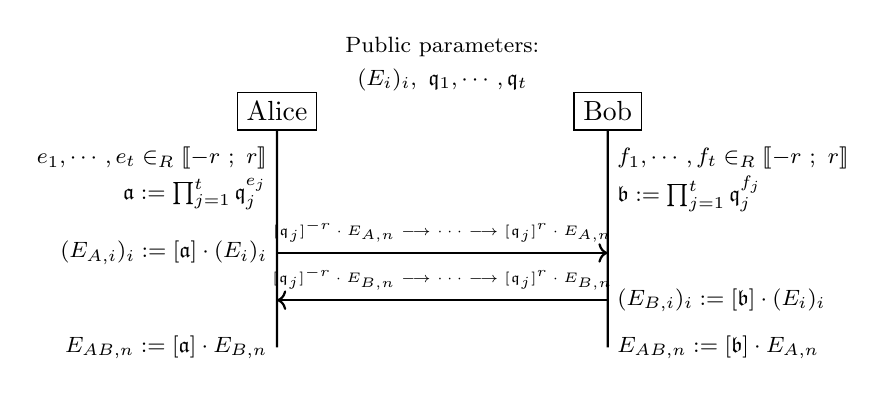
\begin{tikzpicture}[scale=0.6]
  % Public parameter:
  \node[draw=none,fill=none,align=center] (public) at (0,1) {\footnotesize Public parameters:\\\footnotesize $(E_i)_i, \ \mf{q}_1, \cdots, \mf{q}_t$};
  
  % Alice
  \node[draw] (Alice) at (-3.5,0) {Alice}; 
  \draw[thick] (Alice) -- ++(0, -5);
    
  % Calculations of Alice
  \node[draw=none,fill=none,anchor=east] (asecret) at ($(Alice) + (0,-1)$) {\footnotesize $e_1,\cdots, e_t\in_R\i{-r}{r}$};
  \node[draw=none,fill=none,anchor=east] (asecretideal) at ($(Alice) + (0,-1.75)$) {\footnotesize $\mf{a}:=\prod_{j=1}^t\mf{q}_j^{e_j}$};
  \node[draw=none,fill=none,anchor=east] (Apublic) at ($(Alice) + (0,-3)$) {\footnotesize $(E_{A,i})_i:=[\mf{a}]\cdot (E_i)_i$};
  \node[draw=none,fill=none,anchor=east] (akey) at ($(Alice) + (0,-5)$) {\footnotesize $E_{AB,n}:= [\mf{a}]\cdot E_{B,n}$};
    
  % Bob
  \node[draw] (Bob) at (3.5,0) {Bob}; 
  \draw[thick] (Bob) -- ++(0, -5);
   
  % Calculations of Bob
  \node[draw=none,fill=none,anchor=west] (bsecret) at ($(Bob) + (0,-1)$) {\footnotesize $f_1,\cdots, f_t\in_R\i{-r}{r}$};
   \node[draw=none,fill=none,anchor=west] (bsecretideal) at ($(Bob) + (0,-1.75)$) {\footnotesize $\mf{b}:=\prod_{j=1}^t\mf{q}_j^{f_j}$};
  \node[draw=none,fill=none,anchor=west] (Bpublic) at ($(Bob) + (0,-4)$) {\footnotesize $(E_{B,i})_i:=[\mf{b}]\cdot (E_i)_i$};
  \node[draw=none,fill=none,anchor=west] (bkey) at ($(Bob) + (0,-5)$) {\footnotesize $E_{AB,n}:= [\mf{b}]\cdot E_{A,n}$};
   
  % Messages
  \draw[->,thick] ($(Alice)+(0,-3)$) -- ($(Bob)+(0,-3)$) node [pos=0.5,above,font=\footnotesize] {\tiny $[\mfq_j]^{-r}\cdot E_{A,n}\longrightarrow \cdots\longrightarrow [\mfq_j]^{r}\cdot E_{A,n}$};
  \draw[->,thick] ($(Bob)+(0,-4)$) -- ($(Alice)+(0,-4)$) node [pos=0.5,above,font=\footnotesize] {\tiny $[\mfq_j]^{-r}\cdot E_{B,n}\longrightarrow \cdots\longrightarrow [\mfq_j]^{r}\cdot E_{B,n}$};
    
\end{tikzpicture}

\caption{The OSIDH protocol.}
\end{figure}


\end{frame}

\section{Cryptanalysis of OSIDH}

\subsection{Recovering the chain with oriented endomorphisms}

\begin{frame}
\textbf{Recovering the chain with oriented endomorphisms}\footnote[frame]{Onuki (2020).}

\vspace{0.5cm}

\begin{itemize}
\item Given $(E_i)_{i}$ and $(F_i)_{i}:=[\mf{a}]\cdot(E_i)_{i}$, we can recover the secret $[\mf{a}]\in\Cl(\mO_n)$.

\pause

\item \textbf{Problem:} recover $(F_i,\iota_i)_{i}$ with the knowledge of:
\[[\mfq_j]^{-r}\cdot F_{n}\longrightarrow \cdots\longrightarrow [\mfq_j]^{r}\cdot F_{n} \quad (1\leq j\leq t)\]

\pause

\item Assume that we know a $K$-oriented endomorphism $\iota'_n(\beta)\in\End(F_n)$ for some known value $\beta\in\mO_n\setminus\mO_{n+1}$.

\pause

\item Set $\mO_K:=\Z[\theta]$ and $\beta:=a+b\ell^n\theta$ with $b\wedge\ell=1$.

\item We know $\iota'_n(a)=[a]$ so we know $\iota'_n(b\ell^n\theta)$.
\end{itemize}

\pause

\begin{lemma}
$\ker(\iota'_n(b\ell^n\theta))\cap F_n[\ell]=\ker(\widehat{\varphi}'_{n-1})$, with $\varphi'_{n-1}:F_{n-1}\longrightarrow F_n$.
\end{lemma}

\end{frame}

\begin{frame}
\textbf{Recovering the chain with oriented endomorphisms}

\vspace{0.5cm}

\[\xymatrix{
 										      &                     &  & &\\
[\mf{q}_j]^{-r}\cdot F_n \ar[r] & \cdots \ar[r]& F_n \ar[r] & \cdots \ar[r]& [\mf{q}_j]^r\cdot F_n\\
}\]
\end{frame}

\begin{frame}
\textbf{Recovering the chain with oriented endomorphisms}

\vspace{0.5cm}

\[\xymatrix{
 										      &                     & F_{n-1} \ar[d]_{\varphi'_{n-1}} & &\\ 
[\mf{q}_j]^{-r}\cdot F_n \ar[r] & \cdots \ar[r]& F_n \ar@(r,d)[]^{\iota'_n(\beta)} \ar[r] & \cdots \ar[r]& [\mf{q}_j]^r\cdot F_n\\
}\]
\end{frame}

\begin{frame}
\textbf{Recovering the chain with oriented endomorphisms}

\vspace{0.5cm}

\[\xymatrix{
 [\mf{q}_j]^{-r}\cdot F_{n-1} \ar[r] \ar[d] &  \cdots \ar[r] & F_{n-1} \ar[d]_{\varphi'_{n-1}} \ar[r] &\cdots \ar[r] & [\mf{q}_j]^r\cdot F_{n-1} \ar[d]\\ 
[\mf{q}_j]^{-r}\cdot F_n \ar[r] & \cdots \ar[r]& F_n \ar@(r,d)[]^{\iota'_n(\beta)} \ar[r] & \cdots \ar[r]& [\mf{q}_j]^r\cdot F_n\\
}\]
\end{frame}

\subsection{A lattice reduction to find oriented endomorphisms}

\begin{frame}
\textbf{A lattice reduction to find oriented endomorphisms}

\vspace{0.5cm}

\begin{itemize}
\item We look for $\beta\in \mO_n\setminus\mO_{n+1}$ such that $\iota'_n(\beta)$ is easy to compute.

\item We look for:
\[\beta\mO_n=\prod_{j=1}^t (\mf{q}_j\cap\mO_n)^{e_j}\]
with $e_1,\cdots, e_t\in\i{-2r}{2r}$, so that  $\iota'_n(\beta)$ can be inferred from:
\[[\mfq_j]^{-r}\cdot F_{n}\longrightarrow \cdots\longrightarrow [\mfq_j]^{r}\cdot F_{n} \quad (1\leq j\leq t)\]

\item We look for short vectors (of infinity norm $\leq 2r$) in the relations lattice:
\[L:=\left\{(e_1,\cdots,e_t)\in\Z^t \ \middle| \ \prod_{j=1}^t [\mf{q}_j\cap\mO_n]^{e_j}=[1] \quad\mbox{in } \Cl(\mO_n)\right\}\]
\end{itemize}
\end{frame}

\begin{frame}
\textbf{A lattice reduction to find oriented endomorphisms}

\vspace{0.3cm}

\begin{itemize}
\item The relations lattice $L$ can be computed in polynomial time (in $n$ and $t$) because discrete logarithms are easy to compute in $\Cl(\mO_n)$.

\pause 

\begin{lemma}
Heuristically, we have:
\[\(1-\frac{\log\log(t)}{t}\)\frac{|\Cl(\mO_n)|^{1/t}}{2}\leq \lambda_1^{(\infty)}(L)\leq \(1+\frac{\log\log(t)}{t}\)\frac{|\Cl(\mO_n)|^{1/t}}{2}\]
\end{lemma}

\pause 

\item If the key space:
\[\left\{\prod_{j=1}^t [\mf{q}_j\cap\mO_n]^{e_j} \ \middle| \ e_1,\cdots, e_t\in\i{-r}{r} \right\}\]
covers $\Cl(\mO_n)$, then $|\Cl(\mO_n)|\leq (2r+1)^t$ and:
\[\lambda_1^{(\infty)}(L)<2r\]

\item Finding a short vector is exponential but practical with BKZ.
\end{itemize}
\end{frame}

\subsection{Implementation of our attack}

\begin{frame}
\textbf{Implementation with toy parameters:} $\ell=2$, $n=28$,$t=10$, $r=3$ and $K=\Q(i)$.

\begin{columns}[t]
\column{.5\textwidth}
\begin{figure}
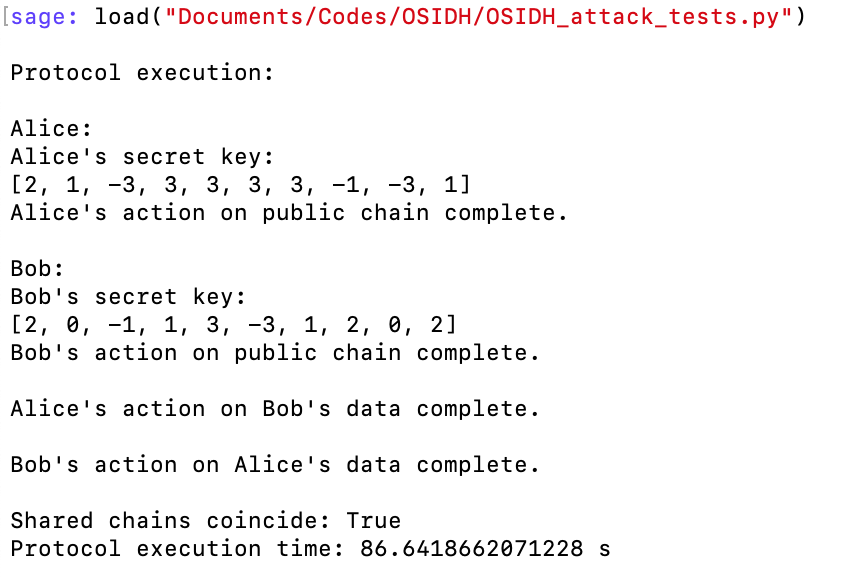
\includegraphics[width=5.5cm]
{Protocol_execution.png} 
\end{figure}


\column{.5\textwidth}

\begin{figure}
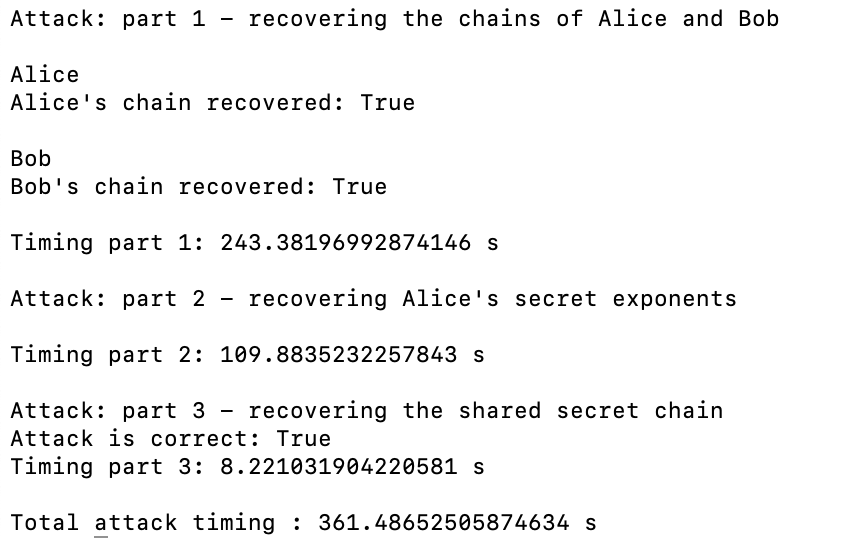
\includegraphics[width=5.5cm]
{Attack_execution.png} 

\end{figure}
\end{columns}

\end{frame}

\begin{frame}
\textbf{Can we scale up the attack?} 

\vspace{0.5cm}

\textbf{Testing lattice reduction:} $\ell=2$, $n=256$,$t=74$, $r=5$ and $K=\Q(i)$.

\begin{itemize}
\item Relations lattice computation: 1h04.
\item Finding a short vector with BKZ: 0.5s.
\item Shortest vector:
\begin{align*}u:=&(-4, 1, 4, 4, -3, 1, 3, 5, 5, 2, 9, 5, 3, 5, -1, 5, -7, 2, -3, 5, 3, -3, 2,\\
&0, 2, 2, 0, -6, -2, -2, -9, 0, -6, 4, 1, -2, 1, 0, 7, 6, -2, -5, -3, -4, \\
&6, -1, 0, -3,-2, -3, 2, 6, 0, 6, -8, -3, -2, -3, 4, 4, -3, -5, 1, 0, \\
&0, 1, -1, 0, 5, -1, -1, 1, -2, -4)\end{align*}
$\|u\|_\infty=9<2r$.
\end{itemize}
\end{frame}

\subsection{Countermeasures}

\begin{frame}
\textbf{Countermeasures:}

\vspace{0.5cm}
\begin{itemize}
\item \textbf{Method 1:} increase $t$ to make it computationally hard to find short vectors.

\item \textbf{Method 2:} make sure that $(2r+1)^t\ll |\Cl(\mO_n)|$, so that:
\[ \lambda_1^{(\infty)}(L)\geq \(1-\frac{\log\log(t)}{t}\)\frac{|\Cl(\mO_n)|^{1/t}}{2}> 2r\]
\pause 
\item Drawbacks of method 1:
\begin{itemize}
\item Increases the protocol complexity by a lot.
\item Diversity: the security relies on a lattice problem.
\end{itemize}
\pause
\item Drawback of method 2: reduces the key space:
\[\left\{\prod_{j=1}^t [\mf{q}_j\cap\mO_n]^{e_j} \ \middle| \ e_1,\cdots, e_t\in\i{-r}{r} \right\}\]
This impedes other cryptographic constructions.
\end{itemize}
\end{frame}

\section{Conclusion}

\begin{frame}
\textbf{To sum up:} Our attack significantly undermines OSIDH:

\vspace{0.3cm}

\begin{itemize}
\item Either OSIDH becomes an inefficient lattice based protocol.

\item Or it no longer satisfies the hypothesis of a cryptographic group action (key space too small).

\end{itemize}

\vspace{0.5cm}
\pause 

\textbf{Future works:}

\vspace{0.3cm}

\begin{itemize}
\item Improve the protocol implementation to scale up the attack.

\item Find a complete cryptanalysis (without countermeasures).

\item Or look for other constructions with the OSIDH framework that can work with a small key space. 
\end{itemize}
\end{frame}

\appendix

\section{Questions}

\begin{frame}
\textbf{Example:} Bob computes $E_{AB,n}=[\mf{b}]\cdot E_{A,n}$ with $[\mf{b}]=[\mf{q}_1]^{f_1}[\mf{q}_2]^{f_2}$.

\[\xymatrix{
[\mf{q}_2]^{f_2}\cdot E_{A,n}  \ar[r] & [\mf{q}_1][\mf{q}_2]^{f_2}\cdot E_{A,n} \ar[r] & \cdots \ar[r] & [\mf{q}_1]^{f_1}[\mf{q}_2]^{f_2}\cdot E_{A,n}\\
[\mf{q}_2]^{f_2-1}\cdot E_{A,n}  \ar[u] \ar[r] & [\mf{q}_1][\mf{q}_2]^{f_2-1}\cdot E_{A,n} \ar[u] \ar[r] & \cdots \ar[r] & [\mf{q}_1]^{f_1}[\mf{q}_2]^{f_2-1}\cdot E_{A,n}\ar[u]\\
\vdots \ar[u] & \vdots \ar[u] & \ddots & \vdots \ar[u]\\
[\mf{q}_2]\cdot E_{A,n}  \ar[u] \ar[r] & [\mf{q}_1][\mf{q}_2]\cdot E_{A,n} \ar[u]\ar[r] & \cdots \ar[r] & [\mf{q}_1]^{f_1}[\mf{q}_2]\cdot E_{A,n} \ar[u] \\
E_{A,n} \ar[u]^{q_2} \ar[r]^{q_1} & [\mf{q}_1]\cdot E_{A,n} \ar[u] \ar[r] & \cdots  \ar[r] & [\mf{q}_1]^{f_1}\cdot E_{A,n}. \ar[u]
}\]

\end{frame}

\end{document}